\documentclass[10pt,a4paper]{article}
\usepackage[utf8]{inputenc}
\usepackage[spanish]{babel}
\usepackage{amsmath}
\usepackage{amsfonts}
\usepackage{amssymb}
\usepackage{graphicx}
\usepackage[left=2cm,right=2cm,top=2cm,bottom=2cm]{geometry}
\usepackage{enumitem}
\usepackage{float}
\setlist[description]{leftmargin=\parindent,labelindent=\parindent}

\begin{document}
\part*{Ejercicio 1}
Se nos pidió diseñar e implementar una maquina de estados capaz de controlar la activación de dos bombas B1 y B2 (simulando su encendido con un LED) que deben mantener el nivel de agua de un depósito que dispone de dos sensores S e I, colados en la parte superior e inferior del depósito, respectivamente. La operatoria de la máquina sigue las siguientes reglas:

\begin{itemize}
\item Si el agua ha superado un sensor, su valor de salida será: 1.
\item Si el deposito estuviera lleno (I=S=1) no se activaría ninguna bomba.
\item Si el deposito estuviera vacío (I=S=0) se activarían ambas bombas.
\item Si el deposito estuviera lleno por la mitad (I=1, S=0) se activaría la ultima bomba en no activarse. 
\end{itemize}

Se nos solicitó tener en cuenta las siguientes consideraciones para la implementación de la maquina de estados:

\begin{itemize}
\item Implementar la solución utilizando tanto una maquina de Mealy como de Moore.
\item Muestre claramente el diagrama de estados y transiciones.
\item Respaldar el diseño con una simulación en Verilog.
\end{itemize} 

\section*{Implementación Maquina de Moore}
\subsection*{Diagrama de Estados y Transiciones}

Se comenzó por la implementación de la máquina de estados de Moore, para ello, se comenzó por realizar un diagrama de estados y transiciones que describa la maquina de estados. Para lo cual se listará primero a las entradas, estados y salidas posibles, y se hará una breve descripción para una mejor comprensión del diagrama.

\subsubsection*{Entradas:}

\begin{description}
\item[Vacío:] Configuración de entrada S=0, I=0, que indica que el depósito se encuentra vacío.
\item[Medio:] Configuración de entrada S=0, I=1, que indica que el depósito esta lleno por la mitad.
\item[Lleno:] Configuracion de entrada S=1, I=1, que indica que el depósito se encuentra lleno.
\end{description}

\subsubsection*{Estados:}

\begin{description}
\item[Ninguna:] Estado que indica que ninguna bomba esta encendida.
\item[Una Sola:] Estado que indica que solo una bomba se encuentra encendida.
\item[Ambas:] Estado que indica que ambas bombas se encuentran encendidas.
\end{description}

\subsubsection*{Salidas:}

\begin{description}
\item[$b_1=0$ y $b_2=0$:] Esta configuración de salida no enciende ninguna bomba.
\item[$b_1=1$,$b_2=0$ o $b_1=0$,$b_2=1$:] Solo se enciende una de las bombas que controla el circuito.
\item[$b_1=1$ y $b_2=1$:] Esta configuración de salida enciende las dos bombas.
\end{description}

A continuación se presenta el diagrama de estados y transiciones, a partir del cual se diseñó la maquina de estados:

\begin{figure}[H]
\centering
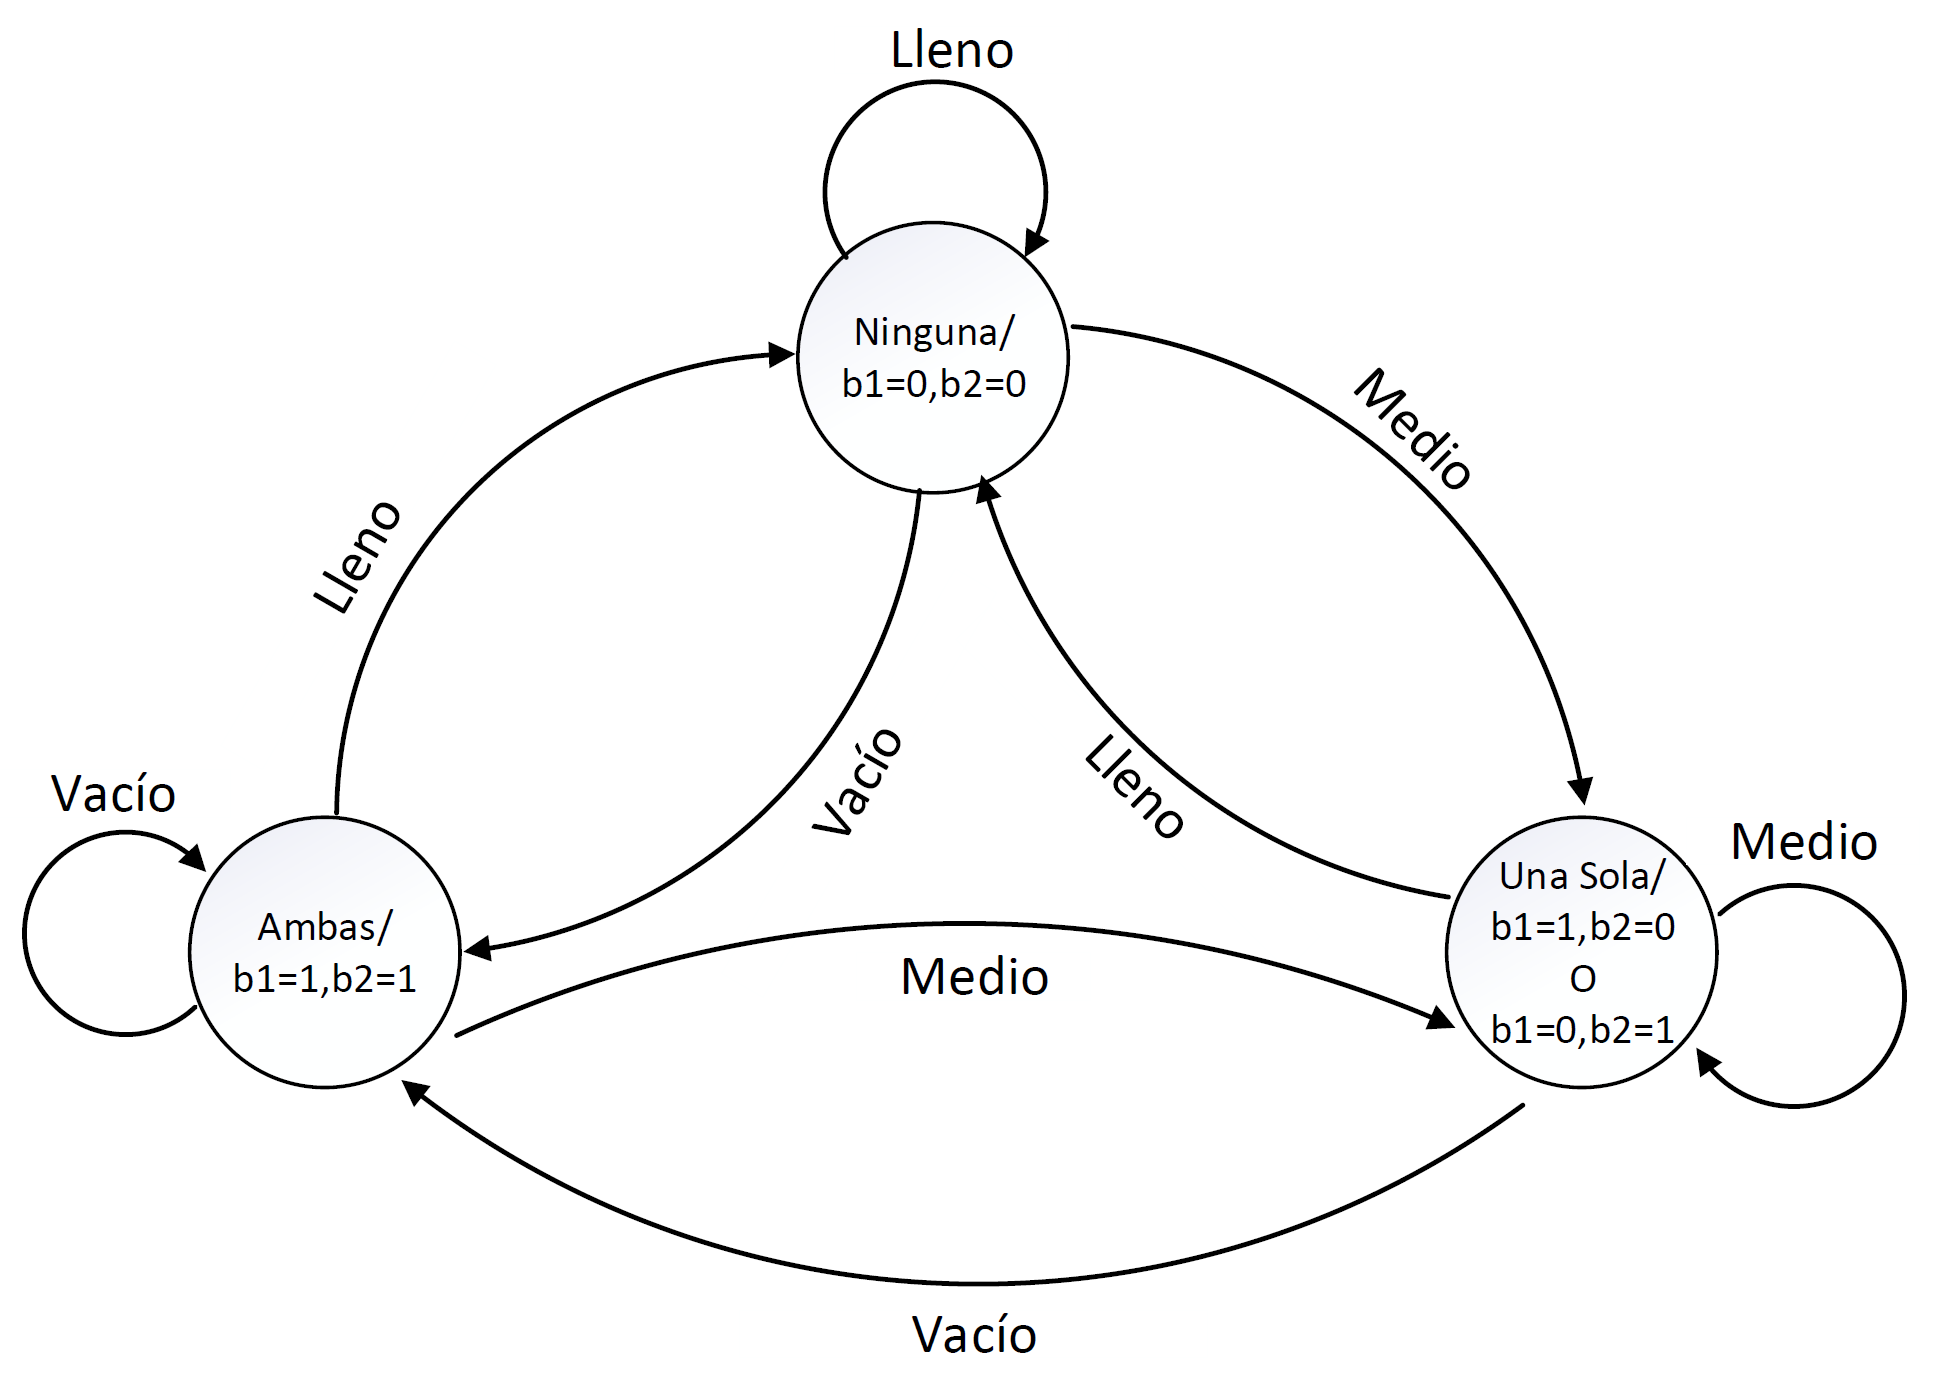
\includegraphics[scale=0.4]{images/diagrama_estados_moore.png}
\caption{Diagrama de estados y transiciones} \label{1_figa}
\end{figure}

Al contar con 3 estados diferentes, mi maquina de estados necesitará como mínimo dos Flip-Flop's para almacenar el estado actual. Los tres estados posibles se codifican a traves de dos variables $y_1$ e $y_0$, de esta forma, tendremos las siguientes configuraciones:

\bigskip

\begin{table}[ht]
	\centering
	\begin{tabular}{c|c}
	Estado & $y_1y_0$ \\ 
	\hline 
	Ninguna & 00 \\ 
	Una Sola & 01 \\ 
	Ambas & 11 \\ 
	\end{tabular} 
\end{table}


Habiendo definido los estados del diseño, se procedió a completar la correspondiente tabla de asignación de estados:
\bigskip
\begin{table}[ht]
	\centering
	\begin{tabular}{c|c|c|c|c}
	Estado Actual & \multicolumn{3}{c|}{Próximo Estado$(Y_1Y_0)$} & Salida\\
	\cline{2-4}
	$(y_1y_0)$ & $SI=00$ & $SI=01$ & $SI=11$ & $(b_1b_2)$\\
	\hline
	00 & 11 & 01 & 00 & 00 \\
	01 & 11 & 01 & 00 & 01 o 10 (Alternado) \\
	11 & 11 & 01 & 00 & 11 \\
	\end{tabular}
	\caption{Tabla de asignación de estados}
	\label{1_t1}
\end{table}

A partir del Cuadro \ref{1_t1} se confeccionó el Cuadro \ref{1_t2}, que implementa la tabla de verdad que determina el próximo estado ($Y_1Y_0$) en función del estado anterior ($y_1y_0$) y las entradas ($SI$). 



\begin{table}[H]
	\centering
	\begin{tabular}{c|c|c}
	$y_1y_0SI$ & $Y_1$ & $Y_0$  \\ 
	\hline 
	0000 & 1 & 1  \\ 
	\hline 
	0001 & 0 & 1  \\ 
	\hline 
	0010 & x & x  \\ 
	\hline 
	0011 & 0 & 0  \\ 
	\hline 
	0100 & 1 & 1  \\ 
	\hline 
	0101 & 0 & 1  \\ 
	\hline 
	0110 & x & x  \\ 
	\hline 
	0111 & 0 & 0  \\ 
	\hline 
	1000 & x & x  \\ 
	\hline 
	1001 & x & x  \\ 
	\hline 
	1010 & x & x  \\ 
	\hline 
	1011 & x & x  \\ 
	\hline 
	1100 & 1 & 1  \\ 
	\hline 
	1101 & 0 & 1  \\ 
	\hline 
	1110 & x & x  \\ 
	\hline 
	1111 & 0 & 0  \\ 
	\end{tabular} 
	\caption{Tabla de verdad cambio de estado}
	\label{1_t2}
\end{table}

Se determinó que es estado $SI=10$ no es una combinación posible, ya que indicaría que el agua ha superado el sensor superior pero no el inferior, lo cual es incompatible con el modelo del deposito, e indicaría un error en los sensores. Como el manejo de errores en el sensores excede los requisitos de la consigna es que se determinó que no son combinaciones posibles y las salidas correspondientes a estas configuraciones se determinaron como 'don't care'

La simplificación mediante Mapas de Karnaugh arrojó los siguientes resultados:

\[
Y_1 = \overline{S}.\overline{I} = \overline{I+S}
\]

\[
Y_0 = \overline{S} = \overline{S + S}
\]

Se observa que el 'próximo estado' no depende del estado actual, sino solamente de las entradas. Se escriben como una negación de suma para luego implementar mediante una compuerta NOR.

\subsection*{Implementación}
\begin{figure}[H]
\centering
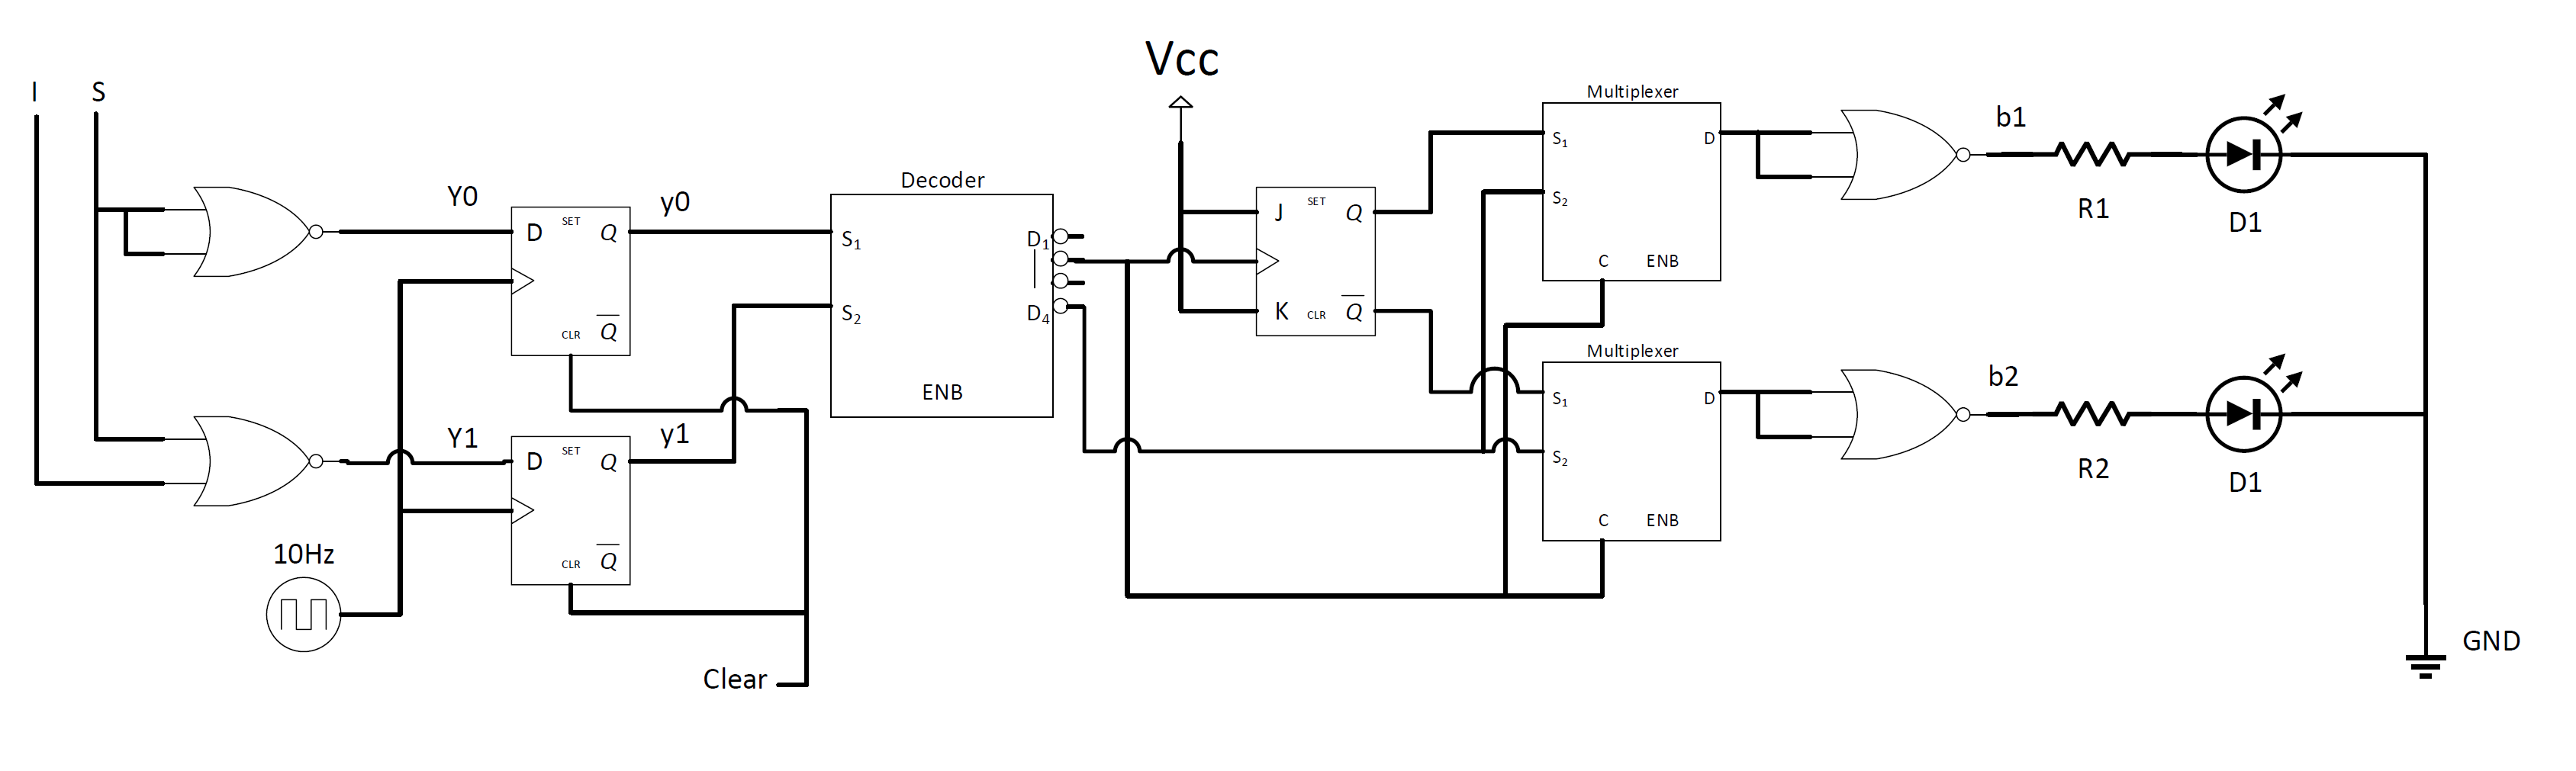
\includegraphics[scale=0.42]{images/diagrama_moore.png}
\caption{Diagrama Esquemático de la Máquina de Estados}
\label{1_fig2}
\end{figure}

La Figura \ref{1_fig2} muestra el circuito implementado. Las salidas de los Flip-Flop's D almacenan el estado actual de la maquina de de estados, mientras que toda la lógica a la salida de estos Flip-Flop's controla las salidas de la máquina.  Se implementó un Flip-Flop JK en modo Toggle para alternar la activación de las bombas cuando solo una de ellas debe activarse. Como se observa, el clock de este Flip-Flop esta controlado por la señal $\overline{Uno Solo}$, la cual valdrá 0 cuando la máquina se encuentre en el estado 'Uno Solo' y valdrá 1 en caso contrario. Cada vez que se produzca una transición del estado 'Uno Solo' hacia otro estado, se invertirán las salidas del Flip-Flop JK. Las salidas $Q$ y $\overline{Q}$ de este Flip-Flop sirven a una de dos entradas de dos multiplexores distintos. La entrada restante esta alimentada por la señal $\overline{Ambas}$, la cual valdrá 0 cuando la máquina se encuentre en el estado 'Ambas'. La señal de selección de ambos multiplexores está controlada por la señal $\overline{Una Sola}$, presentada anteriormente. Así se logra que se alternen las bombas cuando solo una debe encenderse y que se enciendan o apaguen ambas juntas cuando corresponda. Lo que sucede es que la linea de selección de los multiplexores determinan si las bombas tienen el mismo estado o estados complementarios.

\section*{Implementación Maquina de Mealy}
\subsection*{Diagrama de Estados y Transiciones}
Al igual que en el proceso de diseño de la máquina de estados de Moore, el primer paso fue determinar los estados 

\end{document}